\section*{Overview}

The Fenwick tree is the data structure I reach for when the query is really about prefixes and the updates are local.
It is smaller than a segment tree, usually easier to debug, and often exactly right for frequency tables after
coordinate compression.

The usual contest version supports point updates and prefix sums. From that, range sums come for free by subtraction.
With a couple of standard transformations, the same structure also supports range updates or order statistics on a
multiset of counts.

\section*{When to Use It}

Use it when:

\begin{itemize}
  \item the answer over \([l, r]\) can be written as the difference of two prefixes,
  \item updates affect one index at a time, or can be reduced to a few point updates,
  \item you want something lighter than a segment tree,
  \item the array is really a compressed axis of frequencies, counts, or prefix contributions.
\end{itemize}

Typical patterns include inversion counting, sweep-line counting, offline rectangle queries, dynamic frequency tables,
and ``find the k-th active value'' after coordinate compression.

\section*{Core Idea}

For a 1-indexed array, each cell \(\texttt{bit[i]}\) stores the sum of a suffix of the prefix ending at \(i\). The
length of that suffix is the least significant set bit:

\[
\mathrm{lsb}(i) = i \& (-i),
\qquad
\texttt{bit[i]} = \sum_{j=i-\mathrm{lsb}(i)+1}^{i} a_j.
\]

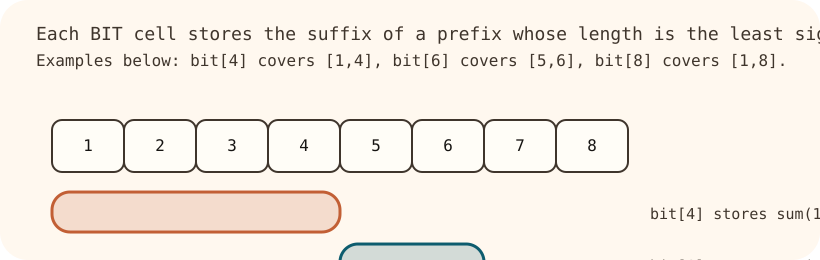
\includegraphics[width=\textwidth]{figures/responsibility.svg}

So \(\texttt{bit[12]}\) covers a chunk of length \(4\), namely \([9, 12]\), because \(\mathrm{lsb}(12) = 4\).
Different indices cover chunks of different lengths, but they fit together in a very structured way.

\paragraph{Worked example.}
Suppose I want the prefix sum up to \(13\). The Fenwick walk visits:
\[
13 \rightarrow 12 \rightarrow 8 \rightarrow 0.
\]
That means the query uses the disjoint buckets \([13,13]\), \([9,12]\), and \([1,8]\). Those intervals are exactly
the full prefix \([1,13]\), with no overlap and no missing position.

\section*{Key Insight}

The two famous transitions
\[
i \mathrel{-}= i \& -i
\quad\text{and}\quad
i \mathrel{+}= i \& -i
\]
are not arbitrary bit tricks. They are the reason the structure works.

\begin{itemize}
  \item In a prefix query, subtracting \(\mathrm{lsb}(i)\) removes the chunk currently owned by \(\texttt{bit[i]}\),
  then jumps to the next disjoint chunk still needed.
  \item In an update, adding \(\mathrm{lsb}(i)\) jumps to the next Fenwick bucket whose responsibility range still
  contains the updated index.
\end{itemize}

So the query walk partitions a prefix into canonical chunks, while the update walk climbs through exactly the buckets
that must be changed.

\section*{Operations / Main Technique}

The standard interface is:

\begin{itemize}
  \item \textbf{add(i, delta)}: add \(\texttt{delta}\) to one position,
  \item \textbf{prefix\_sum(i)}: sum the first \(i\) values,
  \item \textbf{range\_sum(l, r)}: answer by \(\texttt{prefix\_sum(r) - prefix\_sum(l - 1)}\),
  \item \textbf{kth(k)}: on nonnegative frequencies, find the first index whose prefix sum is at least \(k\).
\end{itemize}

\paragraph{Range tricks.}
The three standard variants are worth remembering:

\begin{itemize}
  \item point update + range query: the ordinary tree,
  \item range update + point query: maintain the difference array in one Fenwick tree,
  \item range update + range query: use two Fenwick trees and prefix algebra.
\end{itemize}

I do not memorize the formulas blindly. I remember that Fenwick trees like prefixes, so the trick is always to turn
the desired operation into something prefix-based.

\section*{Correctness Intuition}

The invariant is that every \(\texttt{bit[i]}\) stores one canonical interval ending at \(i\). Those intervals are
chosen so that:

\begin{itemize}
  \item the prefix walk visits disjoint intervals whose union is the queried prefix,
  \item the update walk visits exactly the intervals that contain the updated position.
\end{itemize}

That is enough for correctness.

For queries, nothing is double-counted because the visited intervals are disjoint. Nothing is missed because the walk
stops only after consuming the whole prefix. For updates, every bucket that should contain the position is visited, and
every bucket that should not contain it is skipped.

\section*{Complexity Analysis}

\begin{itemize}
  \item point update: \(O(\log n)\),
  \item prefix query: \(O(\log n)\),
  \item range query: \(O(\log n)\),
  \item k-th query on frequencies: \(O(\log n)\),
  \item memory: \(O(n)\).
\end{itemize}

The logarithm comes from the number of times the least significant set bit can change before the index reaches \(0\)
or leaves the array.

\section*{Implementation}

The reference code keeps the 1-indexed version because I find it easier to reason about than the 0-indexed formulas.
It includes:

\begin{itemize}
  \item \texttt{add},
  \item \texttt{prefix\_sum},
  \item \texttt{range\_sum},
  \item \texttt{kth} for a frequency table.
\end{itemize}

That is already enough for a large fraction of Fenwick tree problems. The main implementation habit is to convert the
external index convention once and then stay consistent everywhere else.

\section*{Common Pitfalls}

\begin{itemize}
  \item Mixing 0-indexed input with a 1-indexed Fenwick implementation.
  \item Calling \texttt{kth} when some frequencies are negative, so prefix sums are no longer monotone.
  \item Forgetting that range sums use \(\texttt{prefix\_sum(l - 1)}\), not \(\texttt{prefix\_sum(l)}\).
  \item Using \texttt{int} when prefix sums can easily exceed \(2^{31} - 1\).
  \item Remembering that ``Fenwick supports range updates'' but forgetting which transformed array is actually stored.
\end{itemize}

\section*{Variants / Extensions}

\begin{itemize}
  \item Two-tree Fenwick for range add and range sum.
  \item Fenwick over frequencies for order statistics.
  \item Multidimensional Fenwick trees for offline geometry or matrix updates.
  \item Fenwick on a different associative group, not just sums, as long as prefix subtraction makes sense.
\end{itemize}

There are also specialized variants for prefix minima under restricted updates, but sums and frequencies are still the
main contest use cases.

\section*{Practice Problems}

\begin{itemize}
  \item Count inversions after coordinate compression.
  \item Maintain a dynamic multiset with insert, erase, and k-th queries.
  \item Offline rectangle counting with a sweep line over one axis and a Fenwick tree over the other.
  \item Problems where range updates can be rewritten as difference-array point updates.
\end{itemize}

\section*{References}

\begin{itemize}
  \item Peter M. Fenwick, \href{https://www.yumpu.com/en/document/view/43186239/a-new-data-structure-for-cumulative-frequency-tables-citeseerx}{A New Data Structure for Cumulative Frequency Tables}.
  \item \href{https://cp-algorithms.com/data_structures/fenwick.html}{cp-algorithms: Fenwick Tree}.
  \item \href{https://atcoder.github.io/ac-library/production/document_en/fenwicktree.html}{AtCoder Library: fenwicktree}.
  \item \href{https://codeforces.com/catalog}{Codeforces Catalog}.
\end{itemize}
